\documentclass[10pt]{beamer}

\usepackage{polyglossia}
\usepackage{csquotes}
\usepackage{datetime}
\usepackage{fontspec}
\usepackage{microtype}
\usepackage{color}
\usepackage{url}
\usepackage{hyperref}
\usepackage{amsfonts}
\usepackage{amsmath}
\usepackage{amsthm}
\usepackage{subcaption}
\usepackage[backend=biber,style=iso-authoryear,sortlocale=en_US,autolang=other,bibencoding=UTF8]{biblatex}
\usepackage{booktabs}
\usepackage{graphics}
\usepackage{pifont}
\usepackage{ulem}
\usepackage{tikz}

\addbibresource{zotero.bib}

\setdefaultlanguage{english}
\setmainfont{TeX Gyre Termes}
\usetheme{Boadilla}
\usecolortheme{crane}
\setbeamertemplate{title page}[default][rounded=true,shadow=false]
\setbeamertemplate{section in toc}[ball unnumbered]
\setbeamertemplate{bibliography item}{}

\hypersetup{
	pdfencoding=auto,
	unicode=true,
	citecolor=green,
	filecolor=blue,
	linkcolor=red,
	urlcolor=blue
}

\makeatletter
\newcommand*{\currentSection}{\@currentlabelname}
\makeatother

\newcommand{\mathmat}{\ensuremath{\mathbf}}

\title[DDny KM FJFI 2021]
{
	Graph Coarsening Can Increase Learning Efficiency
}

\newdate{presentation}{19}{11}{2021}
\date[November 2021]{\displaydate{presentation}}

\author[Marek Dědič]
{
	\underline{Marek~Dědič}\inst{1}\inst{2},
	Martin~Holeňa\inst{3},
	Lukáš~Bajer\inst{2}
}

\institute[FJFI ČVUT]
{
	\inst{1} Faculty of Nuclear Sciences and Physical Engineering, Czech Technical University in Prague \and
	\inst{2} Cisco Systems, Inc. \and
	\inst{3} Institute of Computer Science, Czech Academy of Sciences
}

% TOC
%\AtBeginSection[]{
	%\begin{frame}{\currentSection}
		%\tableofcontents[currentsection]
	%\end{frame}
%}

% Title card
\AtBeginSection[]{
	\begin{frame}
	\vfill
	\centering
	\begin{beamercolorbox}[sep=8pt,center,shadow=true,rounded=true]{title}
		\usebeamerfont{title}\insertsectionhead\par%
	\end{beamercolorbox}
	\vfill
\end{frame}
}

\begin{document}

\begin{frame}
	\titlepage
\end{frame}

% Body

\section{Motivation \& problem being solved}

\begin{frame}{Malware moving infrastructure}
	\begin{itemize}
		\item Malware in the \enquote{wild} sometimes ceases using a particular piece of infrastructure and moves to a different one
		\item Currently, detecting this is very complicated
		\item The aim of this work is to detect a piece of infrastructure going dark and flag the malware sample
		\item As the next step, we would like to predict the new infrastructure the particular malware sample might use and suggest it for manual review
	\end{itemize}
\end{frame}

\begin{frame}{Malware moving infrastructure}
	\begin{figure}
		\centering
		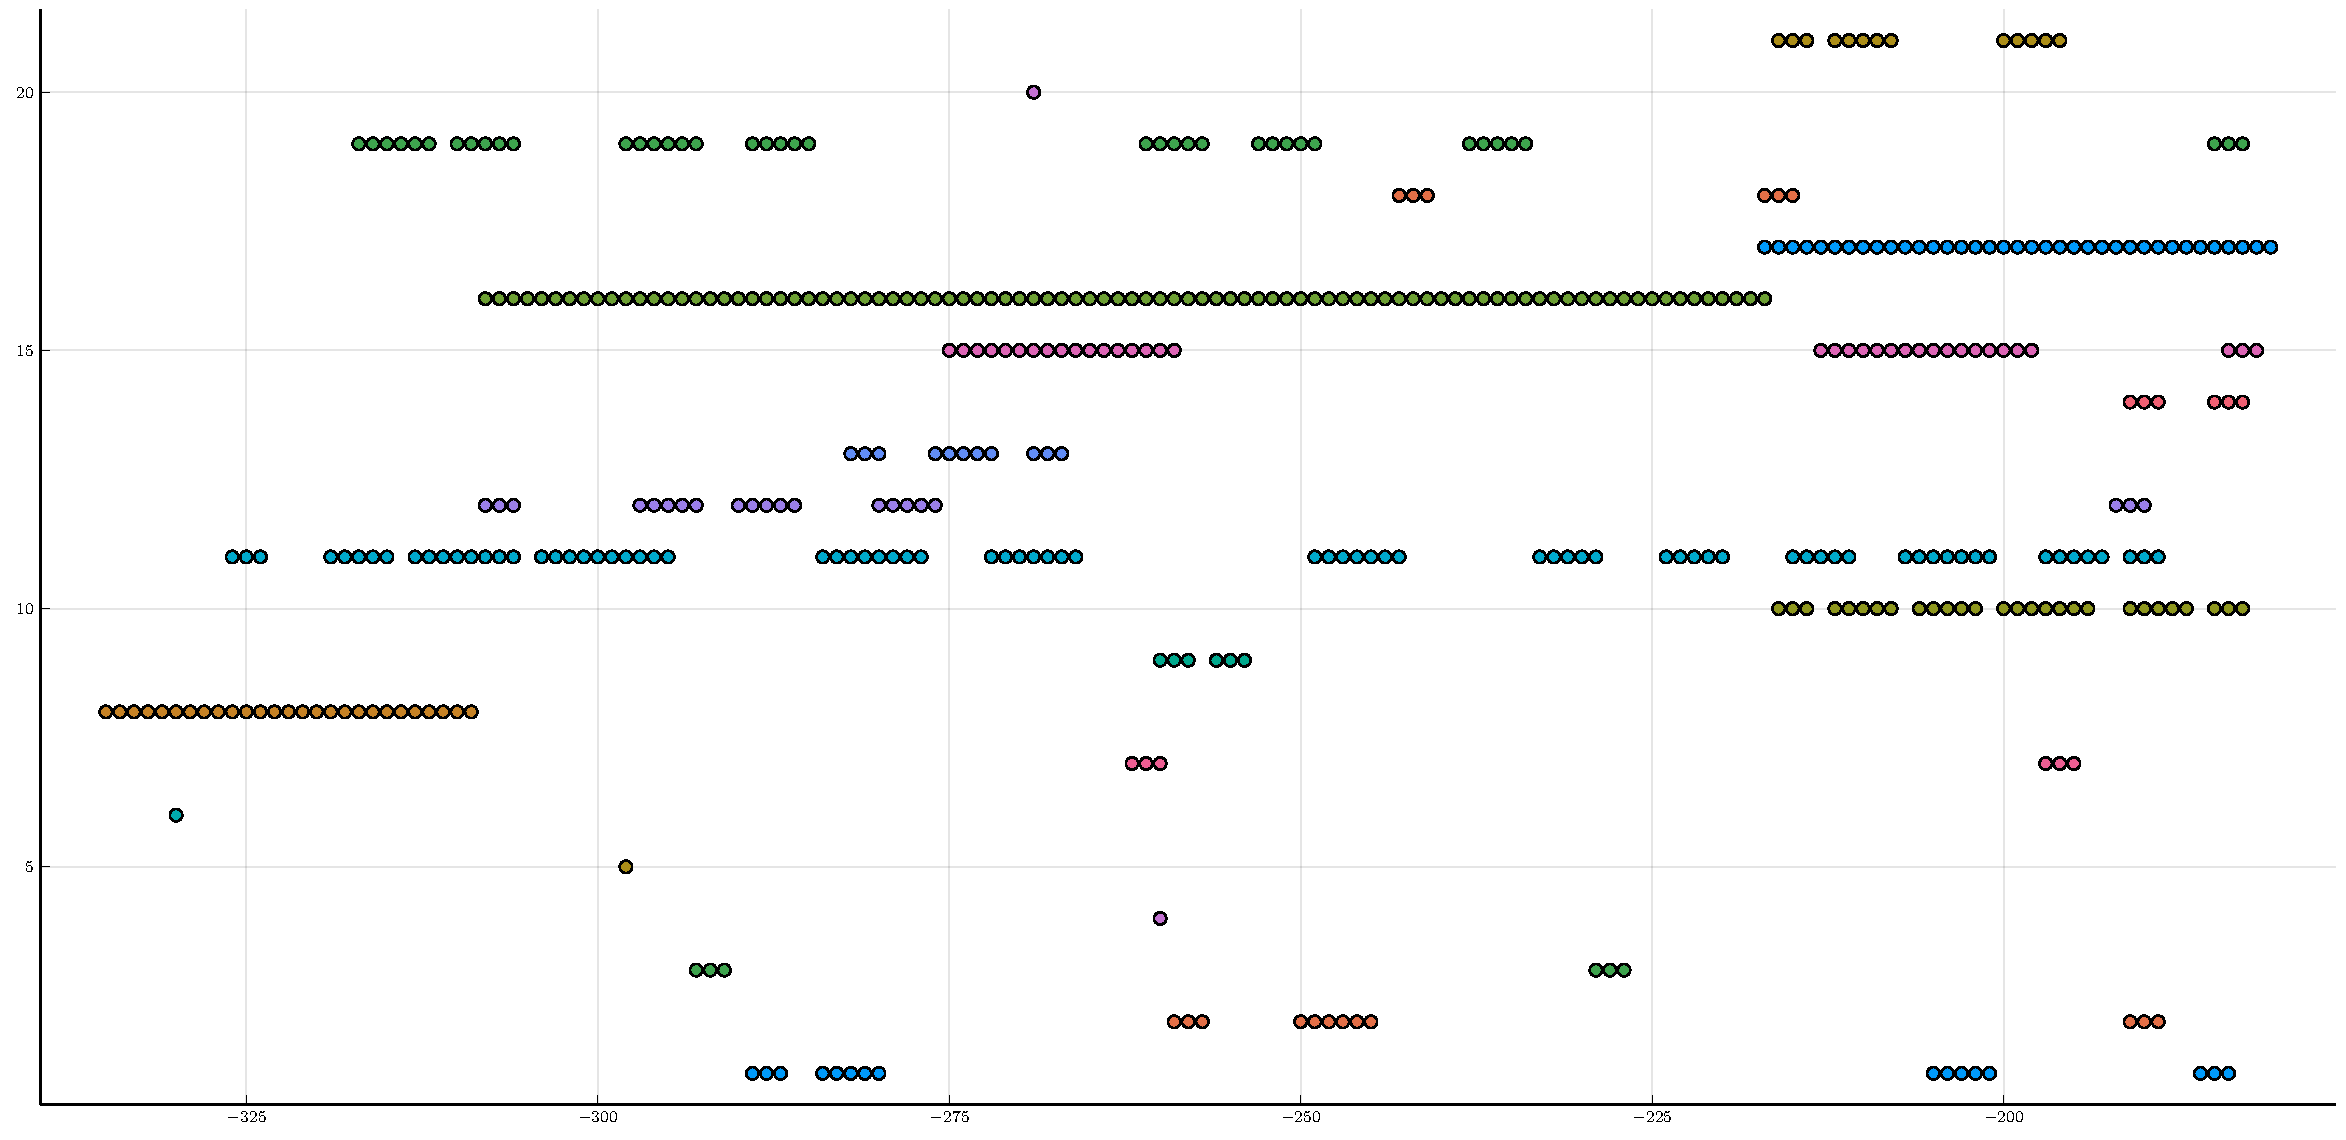
\includegraphics[width=\textwidth]{images/CZAC00-swflows-passivednshostname0/CZAC00-swflows-passivednshostname0.pdf}
		\caption{The usage of different infrastructure by a particular malware sample over time.}
	\end{figure}
\end{frame}

\section{Prior art}

\begin{frame}{HARP - learning on coarser graphs}
	\begin{itemize}
		\item HARP - a method for pretraining on simplified graphs
		\item The simplified graphs are generated in the way depicted bellow
		\item The embedding is trained from the coarsest to the finest graph
	\end{itemize}
	\begin{figure}
		\centering
		\begin{subfigure}[t]{0.38\textwidth}
			\centering
			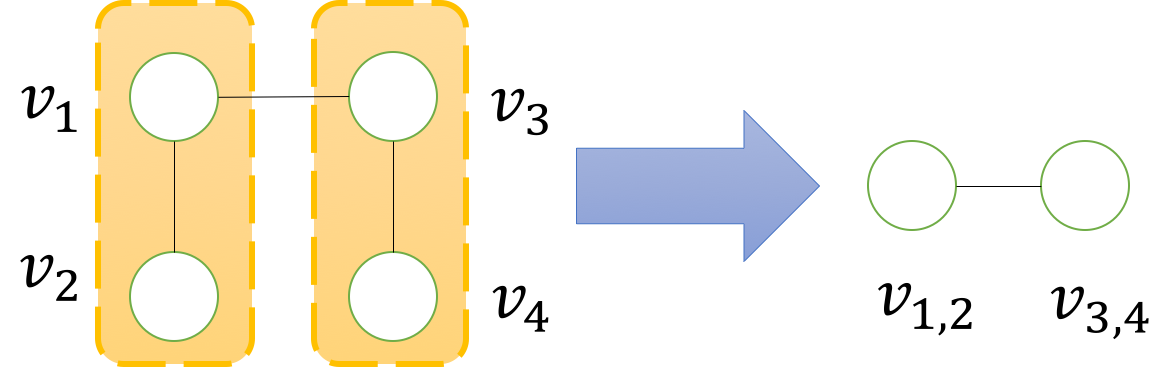
\includegraphics[width=\textwidth]{images/edge_collapsing.png}
			\caption{Edge collapsing}
		\end{subfigure}
		\hspace{2em}
		\begin{subfigure}[t]{0.38\textwidth}
			\centering
			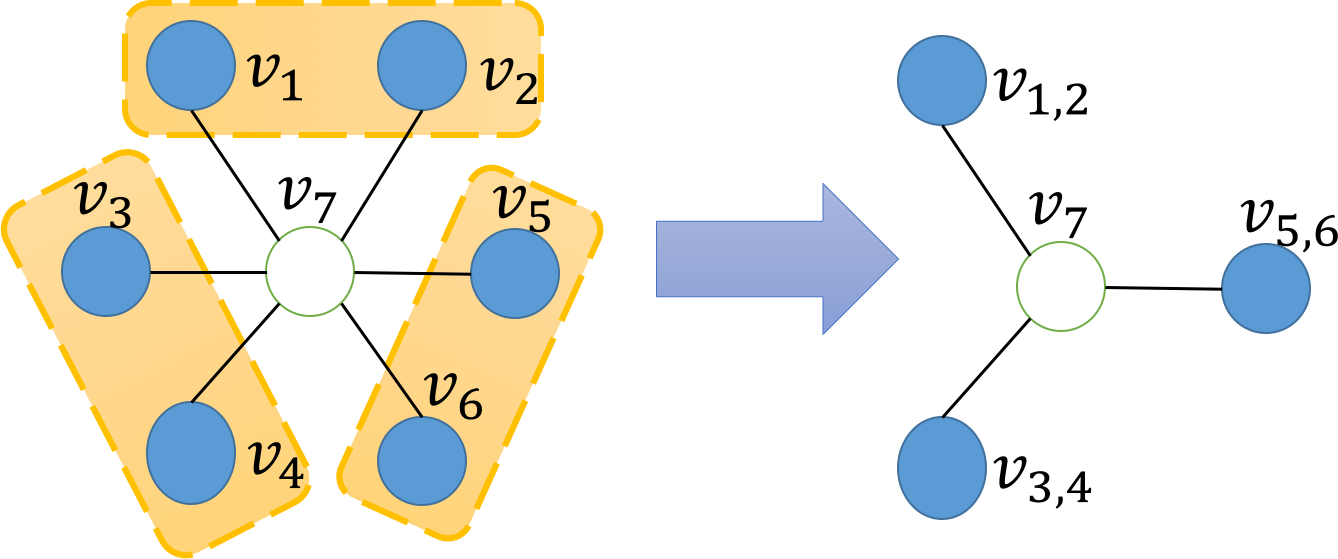
\includegraphics[width=\textwidth]{images/star_collapsing.png}
			\caption{Star collapsing}
		\end{subfigure}
		\caption{HARP coarsening algorithm. \footnote{Images from \cite{chen_harp_2018}.}}
	\end{figure}
\end{frame}

\begin{frame}{Partially injective graph homomorphisms}
	\begin{itemize}
		\item Graph homomorphisms (i. e. subgraph isomorphism)
\[ uv \in E \left( G \right) \implies \varphi \left( u \right) \varphi \left( v \right) \in E \left( H \right) \]
		\item Injective graph homomorphisms (i. e. subgraph isomorphism)
\[ \forall u, v \in V \left( G \right) \quad \varphi \left( u \right) = \varphi \left( v \right) \implies u = v \]
		\item Partially injective graph homomorphisms
\[ \forall uv \in \mathcal{C} \quad \varphi \left( u \right) = \varphi \left( v \right) \implies u = v \]
			where \( \mathcal{C} \subseteq \left( V \left( G \right) \right)^2 \setminus E \left( G \right) \)
	\end{itemize}
\end{frame}

\section{Our work}

\begin{frame}{How do these 2 concepts relate?}
	\begin{itemize}
		\item We can express the HARP transformations as P. I. homomorphisms
		\item The set of all partially injective homomorphisms between 2 graphs forms a lattice, allowing for searching for the coarsening operation tailored to the problem at hand
		\item In this way, you can either preserve or collapse the substructure you are interested in
		\item In the future, the coarsening operation could be learned
	\end{itemize}
\end{frame}

\begin{frame}{Experimental verification of HARP based on PIHom}
	\begin{figure}
		\centering
		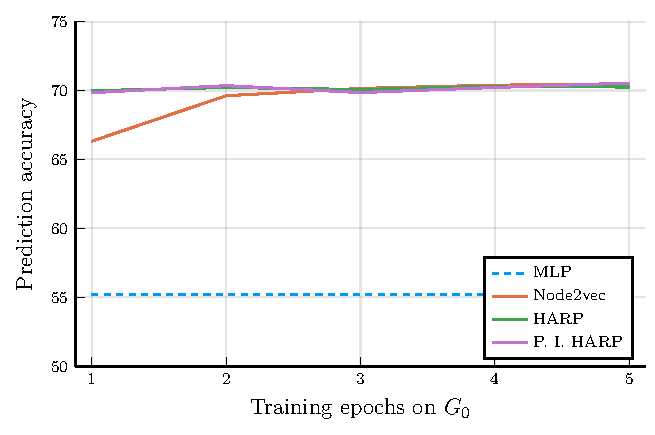
\includegraphics[width=0.8\textwidth]{images/pihom_comparison/pihom_comparison.pdf}
		\caption{Prediction accuracy on OGBN-arxiv}
	\end{figure}
\end{frame}

\begin{frame}{HARP as a complexity-performance trade-off}
	\begin{itemize}
		\item The fact that HARP trains on smaller graphs could be exploited for gains in computational complexity
		\item Experiment: How fast does node2vec train on a graph with and without HARP pretraining?
	\end{itemize}
\end{frame}

\begin{frame}{HARP as a complexity-performance trade-off}
	\begin{figure}
		\centering
		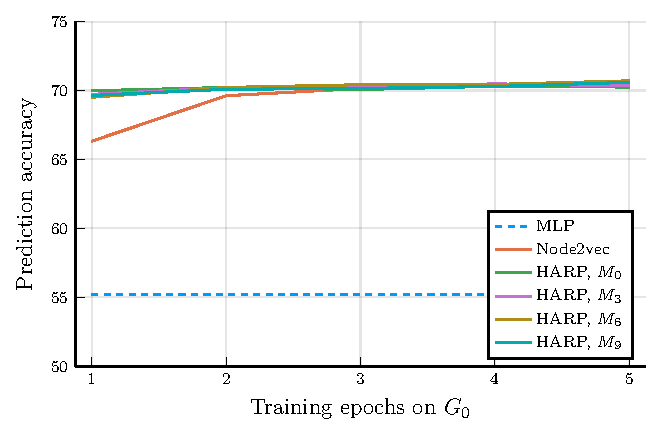
\includegraphics[width=0.8\textwidth]{images/steps_accur/steps_accur.pdf}
		\caption{Prediction accuracy on OGBN-arxiv}
	\end{figure}
\end{frame}

\section{Conclusion}

\begin{frame}{Conclusion}
	\centering
	\begin{itemize}
		\item HARP enables the detection of common subgraphs on large graphs, where other techniques may be computationally unfeasible
		\item Additionally, a new re-formalization of HARP was presented, allowing for a more general approach to graph coarsening
		\item Together, these two innovations enable the use of HARP for malware infrastructure change detection -- the topic of our future work.
	\end{itemize}
\end{frame}

\end{document}
